\documentclass[a4paper,10pt]{article}
\usepackage[utf8]{inputenc}
\usepackage{graphics}
%opening
\title{Guía docente: uso de Dr. Scratch para el desarrollo del pensamiento computacional}
\author{Gregorio Robles, Jesús Moreno, María Luz Aguado, Eva Hu}

\begin{document}

\maketitle

\begin{abstract}

\end{abstract}

\section{Introducción}
En los últimos años estamos presenciando un movimiento global que defiende que el pensamiento computacional debería ser incluido en la formación de todos los niños y niñas, ya que no solo representa un ingrediente vital del aprendizaje de la ciencia, la tecnología, la ingeniería y las matemáticas, sino que es una competencia fundamental para una vida plena en la sociedad digital hacia la que nos dirigimos.

\subsection*{Pero, ¿qué es el pensamiento computacional?}
Jeannette Wing, en su artículo \textit{Computational Thinking}\footnote{https://www.cs.cmu.edu/~CompThink/papers/Wing06.pdf} establece que el ``pensamiento computacional implica resolver problemas, diseñar sistemas y comprender el comportamiento humano, haciendo uso de los conceptos fundamentales de la informática''. Es decir, que la esencia del pensamiento computacional es pensar como lo haría un informático cuando nos enfrentamos a un problema, de manera que podamos aprovechar la potencia de los ordenadores para resolverlos.

Otras definiciones de pensamiento computacional han ido surgiendo en la literatura científica desde entonces. Entre las más aceptadas se encuentran la de Aho\footnote{http://comjnl.oxfordjournals.org/content/55/7/832.abstract} y la de la Royal Society\footnote{https://royalsociety.org/education/policy/computing-in-schools/report/}:
\begin{itemize}
 \item El pensamiento computacional es el proceso que permite formular problemas de forma que sus soluciones pueden ser representadas como secuencias de instrucciones y algoritmos.
 \item El pensamiento computacional es el proceso de reconocimiento de aspectos de la informática en el mundo que nos rodea, y aplicar herramientas y técnicas de la informática para comprender y razonar sobre los sistemas y procesos tanto naturales como artificiales.
\end{itemize}

Una iniciativa muy interesante en relación a la definición del pensamiento computacional es la promovida por la Sociedad Internacional de la Tecnología en la Educación (ISTE) y la Asociación de Profesores de Informática (CSTA), que han colaborado con líderes del mundo de la investigación y la educación superior, la industria y la educación primaria y secundaria para desarrollar una definición operativa\footnote{http://csta.acm.org/Curriculum/sub/CurrFiles/CompThinkingFlyer.pdf} que describa con precisión sus características esenciales y ofrezca un marco de trabajo y un vocabulario común con el que los profesionales de la educación puedan trabajar.

Según esta definición operativa, el pensamiento computacional es un proceso de resolución de problemas que incluye las siguientes características:

\begin{itemize}
 \item Formular problemas de forma que se permita el uso de un ordenador y otras herramientas para ayudar a resolverlos.
 \item Organizar y analizar lógicamente la información.
 \item Representar la información a través de abstracciones como los modelos y las simulaciones.
 \item Automatizar soluciones haciendo uso del pensamiento algorítmico (estableciendo una serie de pasos ordenados para llegar a la solución).
 \item Identificar, analizar e implementar posibles soluciones con el objetivo de lograr la combinación más efectiva y eficiente de pasos y recursos.
 \item Generalizar y transferir este proceso de resolución de problemas para ser capaz de resolver una gran variedad de familias de problemas.
\end{itemize}

\subsection*{Programación informática y pensamiento computacional}
Aunque el pensamiento computacional puede trabajarse desde muchas disciplinas e incluso sin necesidad de contar con dispositivos electrónicos, diversas investigaciones demuestran que la programación informática es una muy buena herramienta para desarrollar esta competencia. (FIXME referencia)

Por consiguiente, responsables educativos de todo el mundo han comenzado a incluir la programación en los curriculum nacionales y regionales. Los ejemplos con mayor repercusión han sido, en el panorama internacional, los de Inglaterra, con una nueva asignatura ``Computing'' obligatoria desde primero de primaria, y Estonia, donde la programación se usa de manera transversal para trabajar diversas asignaturas de primaria y secundaria; y en el caso de España, los de Navarra, que ha incluido la programación en 4º y 5º de primaria asociada al área de matemáticas, y la Comunidad de Madrid, que ha incluido contenidos de programación en la asignatura de tecnología de secundaria y ha creado una asignatura optativa de programación en primaria.

Desde la propia Comisión Europea se está urgiendo a los ministros de la Unión a incluir la programación informática en los planes de estudio para que todos los niños y niñas tengan la oportunidad de desarrollar su pensamiento computacional desde la escuela, ya que estan convencidos de la importancia de esta competencia para la competitividad y la innovación de nuestro continente. (FIXME referencia)En consecuencia, en los próximos años veremos cómo la programación se incluye de forma paulatina en los curriculum de todos los páises europeos, muy probablemente desde la educación primaria.

\subsection*{Cómo trabajar y evaluar el pensamiento computacional}
Sin duda alguna, la inclusión de actividades de programación con \texttt{Scratch}, un lenguaje de programación visual desarrollado específicamente para niños a partir de 6 años, se está implantando en todo el mundo como el estándar para introducir la programación y trabajar el pensamiento computacional en la educación. De hecho, en el momento de escribir este texto, hay más de 8 millones de usuarios registrados en la web de \texttt{Scratch} y más de 11 millones de proyectos compartidos.

No obstante, aunque es posible encontrar rúbricas preparadas por distintas entidades educativas para evaluar el pensamiento computacional del alumnado a partir de los proyectos \texttt{Scratch} desarrollados por los aprendices, no existen apenas herramientas que permitan automatizar parte de este proceso para ayudar a los docentes. En consecuencia, muchos docentes tienen problemas para poder estudiar en profundidad los proyectos de sus alumnos y poder sacar conclusiones para, por ejemplo, aconsejar a sus alumnos acerca de otros bloques que podrían incorporar a sus programas, formar grupos de estudiantes para trabajar un concepto específico que no parecen haber comprendido completamente, o plantearles proyectos avanzados para desarrollar un aspecto concreto una vez alcanzado un determinado nivel. Y este es el motivo que nos llevó a crear la herramienta \texttt{Dr.}{\tiny{ }}\texttt{Scratch}, con el objetivo fundamental de asistir a los docentes en el proceso de enseñanza y evaluación de esta competencia.

\subsection*{Dr. Scratch y el pensamiento computacional}
La herramienta \texttt{Dr.}{\tiny{ }}\texttt{Scratch} permite, entre otras funcionalidades, evaluar el grado de desarrollo del pensamiento computacional a partir de un programa \texttt{Scratch}. Las dimensiones evaluadas son las siguientes:
\begin{itemize}
 \item Abstracción y descomposición de problemas
 \item Nociones de algoritmia y control del flujo de los programas
 \item Pensamiento lógico
 \item Paralelismo
 \item Sincronización
 \item Representación de la información
 \item Interactividad con el usuario
\end{itemize}

\section{Usando Dr. Scratch}

\section{Desarrollando los distintos aspectos del pensamiento computacional con Dr. Scratch}
Para cada una de las dimensiones del pensamiento computacional que \texttt{Dr.}{\tiny{ }}\texttt{Scratch} evalúa, la herramienta asigna una puntuación entre 0 y 3 puntos, en función del grado de desarrollo demostrado en la programación del proyecto analizado. Para aquellas dimensiones en las que existe margen de mejora, \texttt{Dr.}{\tiny{ }}\texttt{Scratch} ofrece información para conocer nuevas posibilidades y seguir mejorando cada uno de estos aspectos.
\subsection{Abstracción y descomposición de problemas}
La capacidad de abstracción y descomposición de problemas te ayuda a dividir un problema en partes más pequeñas que serán más fáciles de comprender, programar y depurar.
\subsubsection{Si has sacado 0 puntos...}
Cuando se comienza a programar con Scratch, en ocasiones puede parecer que la solución más sencilla es programar todo el comportamiento de un personaje en un único programa. Sin embargo, lo ideal es que el comportamiento del personaje sea controlado por diferentes programas y que cada uno de estos programas se ocupe de una cuestión concreta. Veamos un ejemplo:


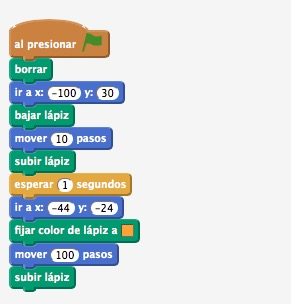
\includegraphics[width=4cm]{img/abs1.jpg}

Este proyecto, que pinta un dibujo en la pantalla, ha sido programado en un único programa que dibuja las dos líneas que componen el dibujo. Aunque es una opción válida, una opción más sencilla de programar y de mantener es dividir el programa en dos partes, de forma que tengamos dos programas diferentes, uno para pintar la primera línea y otro para pintar la segunda:


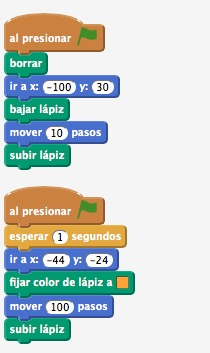
\includegraphics[width=4cm]{img/abs2.jpg}



De este modo, si queremos por ejemplo realizar alguna modificación en una de las líneas dibujadas, es mucho más sencillo saber a qué parte del programa tenemos que dirigirnos para llevar a cabo los cambios.
\subsubsection{Si has sacado 1 punto...}
Scratch permite crear nuevos bloques definidos por los usuarios que se componen de una secuencia de instrucciones. Estas abstracciones permiten crear programas más sencillos de leer, de programar y de mantener. Veamos un ejemplo: 


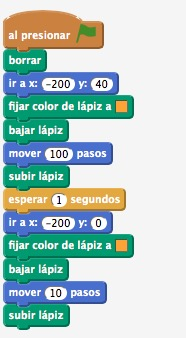
\includegraphics[width=4cm]{img/abs3.jpg}


Este proyecto Scratch dibuja dos líneas naranjas de diferente longitud en la pantalla. En lugar de repetir el código 2 veces, tal como vemos en el ejemplo, es posible definir un bloque “PintaNaranja” que se compone de los bloques que pintan una línea naranja en la pantalla y al que se le puede indicar cuál es la longitud de la línea. Para ello hay que irse a la categoría “Más Bloques” y pulsar en el botón Crear un bloque:


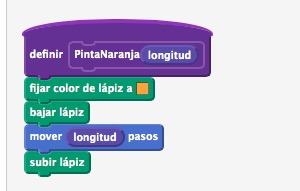
\includegraphics[width=4cm]{img/abs4.jpg}


Una vez definido el bloque “PintaNaranja” es posible utilizarlo en cualquier programa del proyecto, tal como vemos a continuación:


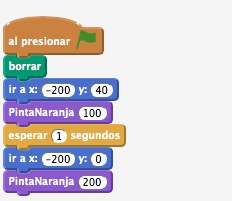
\includegraphics[width=4cm]{img/abs5.jpg}


De este modo, evitamos la repetición de código, lo que hace que nuestros proyectos sean más fáciles de programar y mantener. Tal como se puede observar, la primera vez que se usa el bloque PintaNaranja se le indica una longitud de 100 pasos, mientras que la segunda vez la longitud es de 200 pasos.
\subsubsection{Si has sacado 2 puntos...}

En algunos proyectos Scratch queremos tener muchos personajes iguales que realizan exacatamente las mismas acciones. La primera idea que se nos ocurre para conseguirlo es crear un personaje, programar todo su comportamiento y, una vez que está listo, crear tantas copias como necesitemos. Por tanto, si queremos 20 marcianitos, hay que crear 20 objetos iguales. Sin embargo, ¿qué ocurriría si quiero realizar un cambio en un programa? Tendría que ir objeto por objeto realizando esa modificación.

Para este tipo de situaciones es preferible utilizar clones, un tipo de abstracción que nos ayuda a poder programar un solo objeto, y crear de forma dinámica copias exactas con el mismo comportamiento. 
Veamos cómo funcionan con un ejemplo. Imagina que queremos simular que está nevando en un proyecto. Podemos dibujar un objeto que sea un copo de nive, y una vez que comience la ejecución del proyecto, ir creando clones constantemente que aparezcan en la parte superior de la pantalla y vayan cayendo hasta la parte inferior:

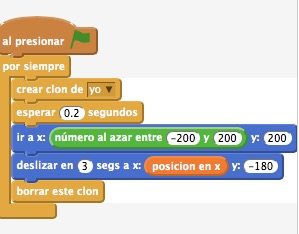
\includegraphics[width=4cm]{img/abs6.jpg}

De este modo, tan solo programando un personaje podemos tener infinitos clones, que se crean en un momento determinado de la ejecución del proyecto y se borran cuando ya no son necesarios.
\subsection{Nociones de algoritmia y control del flujo de los programas}
\subsection{Pensamiento lógico}
\subsection{Paralelismo}
\subsection{Sincronización}
\subsection{Representación de la información}
\subsection{Interactividad con el usuario}

\section{Promoviendo buenos hábitos de programación con Dr. Scratch}
intro
\subsection{Nombrado de objetos}
\subsection{Código muerto}
\subsection{Inicialización de los atributos de los personajes}
\subsection{Repetición de código}

\section{Conclusiones finales}
Es importante mencionar que existen algunos componentes del pensamiento computacional muy importantes, como la depuración de programas, que consiste en la habilidad de localizar y subsanar los errores de los programas, o la capacidad de reinvención, que no pueden ser evaluadas de manera automática al estudiar el código de un proyecto \texttt{Scratch}. Por otra parte, en los entornos educativos los proyectos también pueden ser evaluados en términos de funcionalidad, originalidad o creatividad, aspectos que \texttt{Dr.}{\tiny{ }}\texttt{Scratch} no tiene en cuenta, por lo que los docentes no deben basarse exclusivamente en la puntuación asignada por la herramienta para evaluar el trabajo de sus estudiantes. \texttt{Dr.}{\tiny{ }}\texttt{Scratch} es un recurso para asistir al profesorado en las tareas de evaluación, pero no debe entenderse como un sustituto en este sentido.
\end{document}